	Tous les éléments étant mis en place, j'ai rédigé un guide décrivant les actions à effectuer concernant les tests lors d'une livraison afin de générer les rapports à envoyer à PBI. Celui-ci décrit toutes les étapes pour la création ou modification des tests automatiques ainsi que le travail que j'ai effectué. De plus, celui-ci décrit comment installer et configurer l'ensemble des outils utilisés (TestLink, Apache JMeter et Saxon XSLT).
	
J'ai ensuite pu mettre le guide à disposition des développeurs et leur ai exlicité la marche à suivre finale qui est la suivante :
	\begin{itemize}
		\item Lancer les tests automatiques sur JMeter
		\item Récupérer le fichier XML généré contenant les résultats du plan de test
		\item Exécuter le programme Batch pour générer le fichier XML prêt à l'import pour TestLink
		\item Créer un nouveau plan de test sur TestLink
		\item Importer le fichier XML
		\item Repérer les tests en échecs et créer un ticket Mantis pour ces derniers
		\item Générer les rapports PDF et Excel \\
	\end{itemize}

\begin{figure}[h!]
	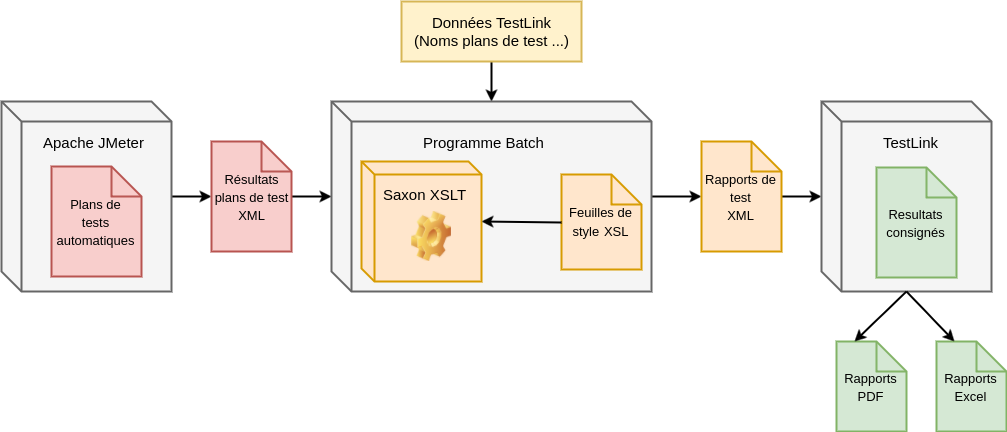
\includegraphics[scale=0.5]{images/travailNeuflizeOBC/testsFonc/testsProcedure.png}
	\centering
	\caption{Procédure de test finale}
	\label{testsProcedure}
\end{figure}

	Lors d'une livraison, une ressource pouvait parfois être occupé jusqu'à une demi-journée rien que pour exécuter l'ensemble des tests et consigner leur résultats, pour les raisons que nous avions évoquées partie \ref{testsFonc_03}. Avec cette nouvelle procédure, la génération des documents à destination du client prenait environ \textbf{10 minutes}, le plus long étant d'attendre la fin de l'exécution des tests automatiques. Ceci représente un gain de temps considérable pour l'équipe et permet d'obtenir des rapports conformes avec les besoins et attentes du client. De plus, cela a permis de soulager les développeurs d'un bon nombre de tâches répétitives et peu intéressantes d'un point de vue technique bien qu'essentielles dans le processus de satisfaction du client, dégageant ainsi du temps supplémentaire dans les sprints pour accomplir les objectifs fixés. \\
	
	Cependant, malgré les bénéfices apportés, certains points restent perfectibles. En effet, l'application web TestLink n'est pas actuellement hébergée sur un serveur dédié. Le projet touchant à sa fin, celui-ci sera repris par une équipe de maintenance qui aura besoin d'accéder à tous les outils et qui devra consigner les résultats de ses tests quotidiens c'est pourquoi il aurait été recommandé de pouvoir procéder à l'installation de TestLink sur un serveur dédié. 
	
	De plus, il aurait pu être intéressant de pousser l'automatisation des tâches à son maximum en ayant recours à Jenkins. En effet, il s'agit d'un outil d'intégration continue permettant d'automatiser différentes procédures. J'ai appris par la suite qu'un Jenkins aurait dû être mis en place au début du projet mais que cela n'avait pas été effectué faute de temps, il est prévu qu'un architecte se charge de cette installation. JMeter et TestLink sont tous deux compatibles avce cet outil tout comme les programmes Batch, il serait ainsi possible par la suite de programmer l'exécution des tests et la création des rapports de manière entièrement automatique à un intervalle de temps souhaité.